\documentclass[conference]{IEEEtran}

\IEEEoverridecommandlockouts % to enable \thanks command to acknowledge SRC support

% *** PACKAGES ***
\usepackage{cite}
\usepackage[pdftex]{graphicx}
\usepackage{amsmath,amssymb,amsfonts}
\usepackage{algorithm}
\usepackage{algorithmic}
\usepackage{array}
\usepackage{subcaption}
\usepackage{overpic}
\usepackage{authblk}
\usepackage[cal=boondox]{mathalpha}

\makeatletter
\def\endthebibliography{%
	\def\@noitemerr{\@latex@warning{Empty `thebibliography' environment}}%
	\endlist
}
\makeatother

%\usepackage{blindtext}
%\usepackage{algorithm2e}

\graphicspath{ {../Figures/} }

\def\BibTeX{{\rm B\kern-.05em{\sc i\kern-.025em b}\kern-.08em
		T\kern-.1667em\lower.7ex\hbox{E}\kern-.125emX}}

\begin{document}
	
	% Title
	\title{Near-Field MIMO-ISAR Millimeter-Wave Imaging}
	
	% Please give the surname of the lead author for the running footer
	\author[1]{Josiah Wayland Smith}
	\author[2]{Muhammet Emin Yanik}
	\author[1]{Murat Torlak}
	\affil[1]{Dept. of Electrical and Computer Engineering, The University of Texas at Dallas, Richardson, TX, United States}
	\affil[2]{Radar and Analytics, Texas Instruments, Dallas, TX, United States}
	
	\maketitle
	
	\begin{abstract}
		
		The use of multiple-input-multiple output (MIMO) millimeter-wave (mmWave) sensors for synthetic aperture radar (SAR) and inverse SAR (ISAR) can aide in overcoming the fundamental challenges of cost-effectiveness and scalability inherent to near-field applications such as concealed item detection and through-wall surveillance. In this paper, prior work done on single-input-single-output mmWave radar systems is extended to the time-delay-multiplexing (TDM) MIMO regime for high-resolution near-field three-dimensional (3-D) imaging. The rotational ISAR (R-ISAR) regime explored in this paper requires rotating the target at a constant radial distance from the transceiver and scanning the transceiver along a vertical track. Using an ultrawideband (UWB) mmWave radar, a high resolution 3-D image can be reconstructed from this two-dimensional scanning taking the spherical nature of the near-field wavefront into consideration. While prior work in literature consists of SISO-ISAR algorithms or computationally inefficient MIMO-ISAR image reconstruction algorithms, this paper describes a novel technique for simple MIMO to SISO phase compensation applied to the R-ISAR regime allowing for use of more efficient SISO-ISAR algorithms. First, an efficient near-field MIMO-ISAR 3-D image reconstruction algorithm is derived based on spherical wave decomposition, circular convolution, and SISO to MIMO phase compensation. This type of spatial-spectral domain analysis provides a more efficient approach than the benchmark back-projection algorithm (BPA), while requiring substantially less computational time. Next, a discussion of several key issues, such as spatial sampling criteria and resolutions, is included. Finally, the proposed algorithm is verified by simulation and experimentally using a prototype 3-D MIMO-ISAR imaging system.
		
		\end {abstract}
		
		\begin{IEEEkeywords}
			millimeter-wave (mmWave), multiple-input multiple-output (MIMO), inverse synthetic aperture radar (SAR), three-dimensional (3-D) imaging.
		\end{IEEEkeywords}
		
		
		%%************************************************************************************
		\section{Introduction}
		\label{sec:introduction}
		%%************************************************************************************
		Over the past several decades, tremendous developments have aided the rapid growth and efficiency of system-on-chip complementary metal oxide semiconductor (CMOS) radio frequency integrated circuits (RFIC). As a result, frequency modulated continuous wave (FMCW) millimeter wave (mmWave) radars have emerged as a cost-effective solution for imaging applications.
		
		Near-field mmWave 3D imaging systems have been demonstrated effective for a host of applications including concealed weapon detection \cite{Sheen:ConcealedWeaponDectection,Zhuge:ConcealedWeaponDectection,Yanik:ConcealedItemImaging}, nondestructive testing \cite{Zhuge:NondestructiveTesting,Baccouche:NondestructiveTesting}, ground penetrating radar \cite{Liu:GPR}. The 3D holographic imaging regime has been investigated in the rectilinear (planar) mode \cite{Yanik:MillimeterWaveNearFieldImaging,Qiao:PlanarSAR} and in cylindrical mode \cite{Sheen:NearField3DRadarImaging}. Additionally, progress has been made towards efficient algorithms for single-input-single-output (SISO) monostatic array synthetic aperture radar (SAR) \cite{Sheen:3DmmWaveImagingSISO} and multi-input-multi-output (MIMO) multistatic array SAR \cite{Zhuge:3DmmWaveImagingMIMO}. Specifically, Gao's work at China's National University of Defense and Technology (NUDT) has demonstrated algorithms for 2-D circular SAR (CSAR) imaging \cite{Gao:CSAR2D} and 3-D MIMO-CSAR imaging \cite{Gao:EfficientAlgorithmMIMOCylindrical}. While SISO-CSAR algorithms proposed by Sheen \cite{Sheen:CSARPatent}, Laviada \cite{Laviada:ECSAR}, Gao, and others are efficient in generating high resolution 3-D holographic images, they fail to account for the multistatic effects from a MIMO array, resulting in aliasing and phase mismatch from the ideal SISO case. In addition, complex MIMO-CSAR algorithms have been developed in attempt to solve such issues; however, these algorithms are computationally expensive and inefficient compared against their SISO counterparts. In this paper, we propose a resolution to this dilemma by leveraging the benefits of MIMO-CSAR, fewer antenna elements and cost efficiency, with the streamlined computational efficiency of the SISO-CSAR algorithms to produce a highly efficient high-resolution 3-D imaging algorithm. Under this MIMO rotation ISAR (R-ISAR) regime, a robust imaging system is prototyped to verify the proposed algorithm and demonstrate its performance.
		
		The rest of this paper is formatted as follows. Section \ref{sec:signal_model} overviews the FMCW signal model, the echo signal from the MIMO rotational ISAR (R-ISAR) scenario shown in Fig. \ref{fig:MIMO_R_ISAR_System_Configuration}, and the multistatic-to-monostatic conversion. Section \ref{sec:derivation_3D_siso_algorithm} contains the derivation for the 3-D image reconstruction algorithm in the SISO R-ISAR regime to be employed once the received echo data has undergone multistatic-to-monostatic phase correction. Section IV proposes a novel efficient 3-D imaging algorithm consisting of key results from Sections \ref{sec:signal_model} and \ref{sec:derivation_3D_siso_algorithm}. Next, Section \ref{sec:key_issues} overviews issues including sampling criteria and spatial resolution. Section \ref{sec:simulations} verifies the proposed algorithm in simulation and discusses its analytical performance. The imaging prototype is described in Section \ref{sec:experimental_setup}. Real 3-D Imaging results are reported in Section \ref{sec:imaging_results}, followed finally by conclusions.
		
		\begin{figure}[h]
			\centering
			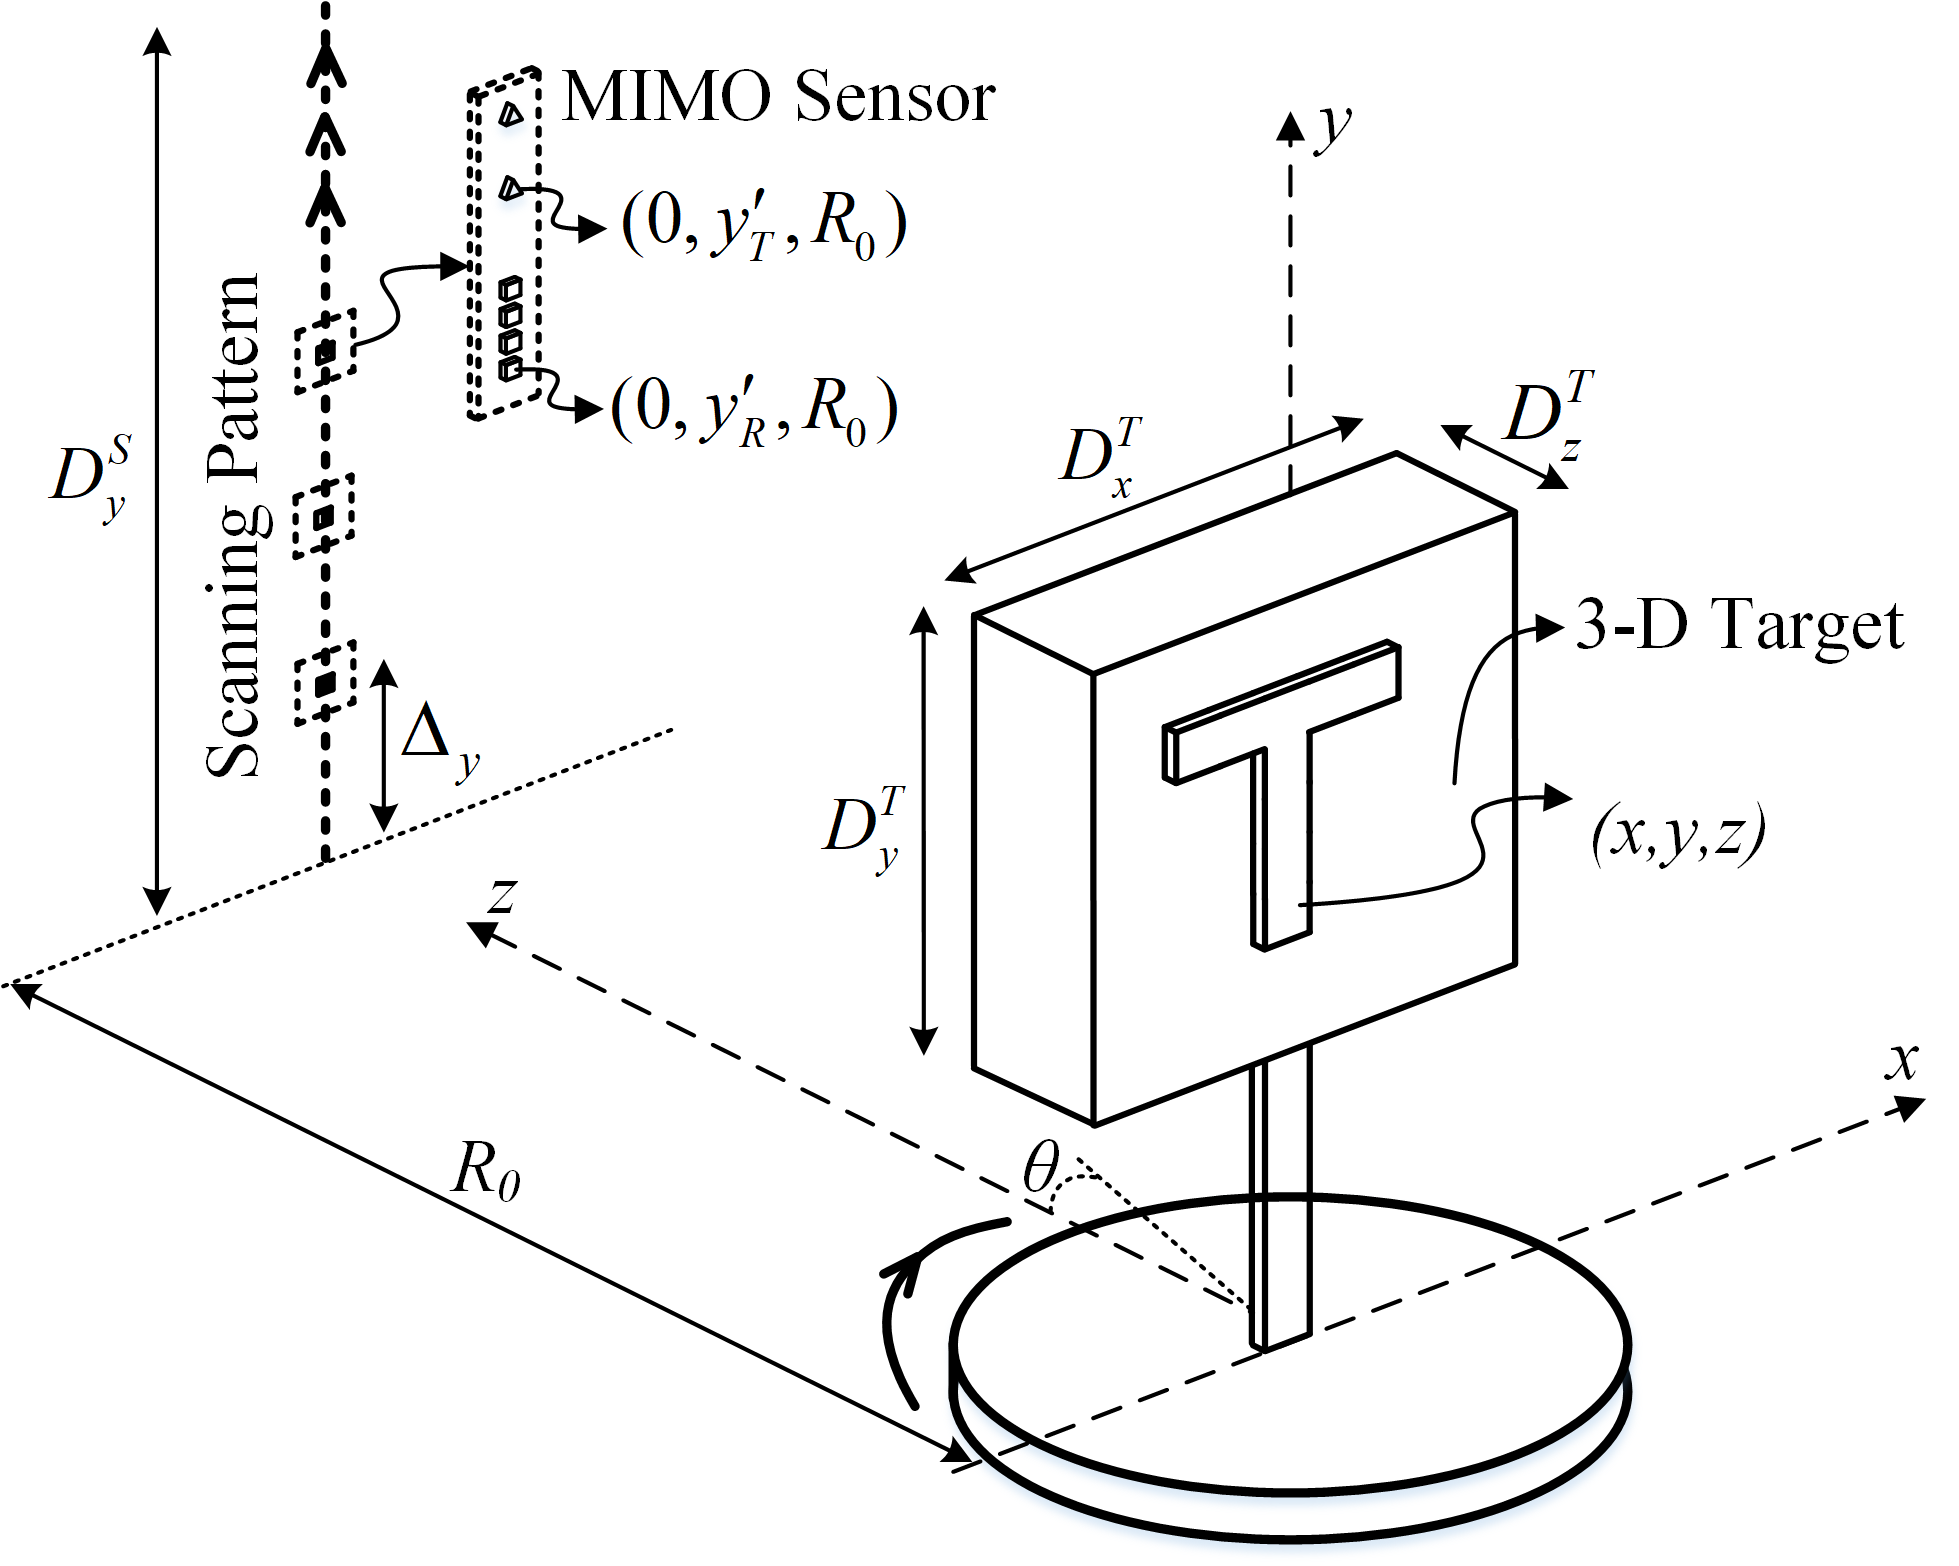
\includegraphics[width=3.4in]{MIMO_R_ISAR_System_Configuration}
			\caption{The geometry of the MIMO R-SAR imaging configuration, where a cylindrical aperture is synthesized by mechanically moving a linear MIMO array vertically and rotating the target.}
			\label{fig:MIMO_R_ISAR_System_Configuration}
		\end{figure} 
		
		
		%%************************************************************************************
		\section{FMCW Signal Model}
		\label{sec:signal_model}
		%%************************************************************************************
		The FMCW chirp waveform has emerged as an excellence choice for mmWave sensors, offering numerous advantages including large bandwidth and affordability. The FMCW signal model for a single MIMO transmitter (Tx) receiver (Rx) pair is examined in this section.
		
		First, consider the transmitted FMCW signal.
		
		\begin{equation}
		m(t) = e^{j2\pi(f_0t + 0.5Kt^2)} , 0 \leq t \leq T,
		\label{Eq_fmcw_signal}
		\end{equation} 
		where $f_0$ is the chirp start frequency at time 0, $K = B/T$, is the slope of the chirp, $B$ is the bandwidth, $T$ is the chirp duration, and $t$ is the fast time variable.
		
		Assuming an ideal point reflector located at the point $(x,z,y)$, with the Tx/Rx pair located in a colinear vertical array at the points $(x',z',y_T')$ and $(x',z',y_R')$ respectively, the return signal can be modeled by
		
		\begin{equation}
		\tilde{s}(t) = \sigma m(t-\tau) = \sigma e^{2\pi(f_0(t-\tau)+0.5K(t-\tau)^2)},
		\end{equation}
		where $\tau = (R_T+R_R)/c$ is the round trip time delay, $c$ is the speed of light, $\sigma = p/(R_T R_T)$ is the combined complex reflectivity of the point reflector $p$ and the round trip amplitude decay. The received signal $\tilde{s}(t)$ is demodulated with the transmitted signal $m(t)$ to reduce the required sample rate, while maintaining the phase information from which the range of each target can be extracted. This process is known as dechriping and yields the beat signal as
		
		\begin{equation}
		s(t) = \sigma e^{2\pi(f_0\tau + K\tau t - 0.5 K \tau^2)}.
		\label{Eq_beat_signal_exp}
		\end{equation}
		
		The last term in the complex exponential is known as the residual video phase (RVP) and in near-field applications is negligible. Now, the complex beat signal can be rewritten in the wavenumber domain as
		\begin{equation}
		s(k) = p \frac{e^{j2k(R_T+R_R)}}{R_T R_R}, \frac{2\pi f_0}{c} \leq k\leq \frac{2\pi f_t}{c},
		\end{equation}
		where $f_T = f_0 + KT$ is the end frequency of the chirp. The relative ranges can be computed easily by
		
		\begin{align}
		\begin{split}
		R_T = \sqrt{(x - x')^2 + (z - z')^2 + (y - y_T')^2}, \\
		R_R = \sqrt{(x - x')^2 + (z - z')^2 + (y - y_R')^2}.
		\end{split}
		\end{align}
		
		It has been shown in \cite{Yanik:NearFieldMIMOSAR,Yanik:CascadedMIMO}, for small $d_y$, the distance between transmitter and receiver elements, the signal $s(k)$ for the $\mathcal{l}^{th}$ pair can be approximated by
		
		\begin{equation}
		s_\mathcal{l}(k) \approx p \frac{e^{j2k\hat{R} + j\phi_\mathcal{l}(k)}}{\hat{R^2}} = \hat{s}_\mathcal{l}(k) e^{j\phi_\mathcal{l}(k)},
		\end{equation}
		where
		\begin{align}
		\hat{s}_\mathcal{l}(k)& = p \frac{e^{j2k\hat{R}}}{\hat{R^2}}, \\
		\phi_\mathcal{l}(k) &= k\frac{d_y^2}{4R_0}.
		\label{Eq_multistatic_signal}
		\end{align}
		
		In (\ref{Eq_multistatic_signal}), $\hat{R}$ is the distance from the midpoint between the transmitter and receiver pair to the point reflector, $\hat{s}_\mathcal{l}(k)$ is the virtual SISO signal from the virtual element located at the midpoint of the transmitter and receiver pair, $\phi_\mathcal{l}(k)$ is the phase difference from the multistatic nature of the MIMO pair, and $R_0$ is the reference distance from the dimension across which the MIMO pair is scanned and the target location. For the R-ISAR scenario, the scanning radius serves this purpose.
		
		Now, the virtual SISO signal can be approximated by the received MIMO echo signal by
		\begin{equation}
		\hat{s}_\mathcal{l}(k) = s_\mathcal{l}(k)e^{-j\phi_\mathcal{l}(k)}.
		\end{equation}
		
		
		%%-----------------------------------------------------------------------------------------
		\subsection{MIMO Rotational ISAR (R-ISAR) Echo Signal}
		\label{Sec_mimo_r-isar_signal}
		
		The R-ISAR scenario, as shown in Fig. 1, consists of a rotational scanner whose center is the origin and a MIMO array scanned along the y-axis (vertically), and located at a constant distance of $R_0$ from the center of the rotator. The position of the transmitter and receiver pair from each point in the target domain $(x,z,y)$ depends on the rotation angle $\theta$ and the distance $R_0$.
		
		\begin{align}
		\begin{split}
		R_T = \sqrt{(x - R_0 cos\theta)^2 + (z - R_0 sin\theta)^2 + (y - y_T')^2}, \\
		R_R = \sqrt{(x - R_0 cos\theta)^2 + (z - R_0 sin\theta)^2 + (y - y_R')^2}.
		\end{split}
		\end{align}
		
		Now, the MIMO echo signal from the R-ISAR scenario can be modeled as:
		\begin{equation}
		\label{Eq_mimo_echo_signal}
		s(\theta,k,y_T',y_R') = \iiint \frac{p(x,z,y)}{R_T R_R} e^{jk(R_T + R_R)} dx dz dy.
		\end{equation}
		
		
		%%-----------------------------------------------------------------------------------------
		\subsection{Multistatic-to-Monostatic Conversion}
		\label{Sec_multistatic_to_monostatic_conversion}
		
		Using the derivations provided in this section, the received echo data from the multistatic MIMO array undergo a simple transformation to approximate its counterpart echo signal from the virtual-SISO array elements. To convert this 4-D MIMO signal to a 3-D virtual-SISO signal, the following phase compensation is performed \cite{Yanik:CascadedMIMO},
		
		\begin{equation}
		\label{Eq_phase_compensation}
		\hat{s}(\theta,k,y') = s(\theta,k,y_T',y_R') e^{-jk\frac{d_y^2}{4R_0}}.
		\end{equation}
		
		This compensation is a crucial step in the algorithm. By compensating the phase of the multistatic MIMO signal to obtain an approximate of the echo signal from virtual elements located at the midpoint of each MIMO transmitter/receiver pair, this virtual-SISO data can be fed into the efficient 3-D imaging algorithm derived in section \ref{sec:derivation_3D_siso_algorithm}.
		
		%%************************************************************************************
		\section{Derivation of 3-D Image SISO Reconstruction Algorithm}
		\label{sec:derivation_3D_siso_algorithm}
		%%************************************************************************************
			
		Using the R-ISAR scenario shown in Fig. 1, the return signal from a monostatic SISO transceiver, neglecting amplitude terms, can be modeled as
		
		\begin{equation}
		\hat{s}(\theta,k,y') = \iiint p(x,z,y) e^{j2kR} dx dz dy,
		\end{equation}
		where
		
		\begin{equation}
		R = \sqrt{(x - R_0cos\theta)^2 +  (z - R_0sin\theta)^2 + (y - y')^2},
		\end{equation}
		and $p(x,z,y)$ is the complex reflectivity function of the target scene. Using the method of stationary phase (MSP), the exponential term in (15) can be decomposed as
		
		\begin{align}
		\begin{split}
		&e^{j2k\sqrt{(R_0cos\theta - x)^2 + (R_0sin\theta - z)^2 + (y - y')^2}} = \\ 
		&\iint e^{jk_rcos\phi(R_0cos\theta - x) + jk_rsin\phi(R_0sin\theta - z) + jk_{y'}(y-y'))} d\phi dk_{y'},
		\end{split}
		\label{}
		\end{align}
		where the angle of each plane wave component in the $x-z$ plane is $\phi \in [-\pi/2,\pi/2]$, and $k_{y'}$ is the y-component of the wavenumber bounded by $k_{y'} \in [-2k,2k]$. Using the dispersion relation
		
		\begin{equation}
		4k^2 = k_x^2 + k_y^2 + k_z^2,
		\end{equation}
		we define $k_r$ as the wavenumber component in the $x-z$ plane as
		
		\begin{equation}
		\label{Eq_stolt_1}
		k_r = \sqrt{k_x^2+k_z^2} = \sqrt{4k^2 - k_y^2}.
		\end{equation}
		
		Combining the above relations yields
		\begin{align}
		\begin{split}
		\hat{s}(&\theta,k,y') = \\
		& \iint \left[ \iiint p(x,z,y)e^{-j(k_rcos\phi)x-j(k_rsin\phi)z-jk_{y'}y}dxdydz \right] \\
		& \times e^{jk_rRcos(\theta-\phi) + jk_{y'}y'} d\phi dk_{y'},
		\end{split}
		\label{Eq_mimo_r_isar_signal_expanded}
		\end{align}
		
		The term inside the $[\bullet]$ brackets is the three-dimensional Fourier transform of the reflectivity function. Using the following Fourier transform pair
		
		\begin{equation}
		p(x,z,y) \iff P(k_rcos\phi,k_rsin\phi,k_y),
		\end{equation}
		(\ref{Eq_mimo_r_isar_signal_expanded}) yields
		\begin{align}
		\begin{split}
		\hat{s}(\theta,k,y') &= \iint e^{jk_rRcos(\theta-\phi)} \\
		&P(k_rcos\phi,k_rsin\phi,k_y) e^{jk_{y'}y'}d\phi dk_{y'}.
		\end{split}
		\label{Eq_mimo_r_isar_signal_expanded_2}
		\end{align}
		
		Taking the Fourier transform with respect to $y'$ on both sides and dropping the distinction between $z'$ and $z$ due to coincidence of the domains:
		
		\begin{equation}
		\hat{S}(\theta,k,k_y) = \int_{-\frac{\pi}{2}}^{\frac{\pi}{2}} e^{jk_rRcos(\theta-\phi)} P(k_rcos\phi,k_y,k_rsin\phi)d\phi. 
		\end{equation}
		
		Define:
		
		\begin{align}
		\label{Eq_mimo_r_isar_signal_expanded_3}
		\hat{P}(\phi,k_r,k_y) &\triangleq P(k_rcos\phi,k_rsin\phi,k_y) \\
		g(\theta,k_r) &\triangleq e^{jk_rR_0cos\theta}.
		\end{align}
		
		Now:
		
		\begin{equation}
		\hat{S}(\theta,k,k_y) = \int_{-\frac{\pi}{2}}^{\frac{\pi}{2}} g(\theta-\phi,k_r) \hat{P}(\phi,k_r,k_y)d\phi, 
		\end{equation}
		which represents a convolution in the $\theta$ domain:
		
		\begin{equation}
		\hat{S}(\theta,k,k_y) = g(\theta,k_r) \circledast_\theta \hat{P}(\theta,k_r,k_y),
		\end{equation}
		where $\circledast_\theta$ is the convolution operator along the $\theta$ domain.
		
		Taking the Fourier transform across the $\theta$ domain on both sides yields:
		
		\begin{equation}
		\hat{S}(\Theta,k,k_y) = G(\Theta,k_r)\tilde{P}(\Theta,k_r,k_y),
		\end{equation}
		where
		
		\begin{align}
		G(\Theta,k_r) &= FT_{1D}^{(\theta)}[g(\theta,k_r)],\\
		\tilde{P}(\Theta,k_r,k_y) &= FT_{1D}^{(\theta)}[\hat{P}(\theta,k_r,k_y)]
		\end{align}
		
		Solving for $\tilde{P}$ by taking the inverse filter $G^*(\Theta,k_r)$ and then taking an inverse Fourier transform across the $\Theta$ domain for both sides to obtain $\hat{P}$:
		
		\begin{align}
		\tilde{P}(\Theta,k_r,k_y) &= \hat{S}(\Theta,k,k_y)G^*(\Theta,k_r), \\
		\hat{P}(\theta,k_r,k_y) &= IFT_{1D}^{(\Theta)}\left[ \hat{S}(\Theta,k,k_y)G^*(\Theta,k_r) \right]
		\end{align}
		
		By (\ref{Eq_mimo_r_isar_signal_expanded_3}):
		
		\begin{equation}
		P(k_r cos\theta,k_r sin\theta,k_y) = IFT_{1D}^{(\Theta)}\left[ \hat{S}(\Theta,k,k_y)G^*(\Theta,k_r) \right],
		\end{equation}
		where $k_x = k_r cos\theta$ and $k_z = k_r sin\theta$. $\hat{P}$ will be a non-uniformly sampled function of $\theta$ and $k_r$ and will need to be interpolated onto a uniform $(k_x,k_z,k_y)$ grid via Stolt interpolation using the equation (19) and the following relations:
		
		\begin{align}
		\label{Eq_stolt_2}
		\theta &= tan^{-1}\left(\frac{k_z}{k_x}\right), \\
		\label{Eq_stolt_3}
		k &= \frac{1}{2}\sqrt{k_x^2 + k_y^2 + k_z^2}.
		\end{align}
		
		The Stolt interpolation process will be denoted by the $\mathcal{S}[\bullet]$ operator, such that:
		\begin{equation}
		P(k_x,k_z,k_y) = \mathcal{S}[P(k_r cos\theta,k_r sin\theta,k_y)].
		\end{equation}
		
		Finally, the algorithm can be summarized by (\ref{Eq_risarAlgoSummary_1}) and (\ref{Eq_risarAlgoSummary_2}).
		\begin{align}
		\label{Eq_risarAlgoSummary_1}
		p(x,z,y) &= IFT_{3D}^{(k_x,k_z,k_y)}\left[ P(k_x,k_z,k_y) \right], \\
		\label{Eq_risarAlgoSummary_2}
		P(k_x,k_z,k_y) &= \mathcal{S}\left[IFT_{1D}^{(\Theta)}\left[ FT_{2D}^{(\theta,y)}\left[\hat{s}(\theta,k,y)\right]G^*(\Theta,k_r)\right]\right].
		\end{align}
		
		
		%%************************************************************************************
		\section{Proposed 3-D Image MIMO Reconstruction Algorithm}
		\label{sec:3D_mimo_algorithm}
		%%************************************************************************************
		
		Combining the results from Section \ref{sec:signal_model} and \ref{sec:derivation_3D_siso_algorithm}, the complete multistatic-to-monostatic 3-D image reconstruction algorithm can be written as the following.		
		
		\textbf{Efficient MIMO R-ISAR 3-D Holographic Imaging Algorithm}
		\begin{enumerate}
			\item Gather the raw MIMO echo data as $s(\theta,k,y_T,y_R)$.
			\item Perform the phase compensation described in (\ref{Eq_phase_compensation}) to acquire $\hat{s}(\theta,k,y)$.
			\item Perform a 2-D FFT across the $\theta$ and $y$ dimensions of the phase corrected data to obtain $\hat{S}(\Theta,k,k_y)$.
			\item Generate the azimuth filter $g(\theta,k_r) \triangleq e^{jk_rR_0cos\theta}$ and implement an FFT across the $\theta$ dimension to compute the spectral azimuth filter $G(\Theta,k_R)$
			\item Multiply $\hat{S}(\Theta,k,k_y)$ by the inverse filter $G^*(\Theta,k,k_y)$  and perform an IFFT across the $\Theta$ domain to obtain $P(k_rcos\theta,k_rsin\theta,k_y)$.
			\item Apply Stolt interpolation using the relations in (\ref{Eq_stolt_1}), (\ref{Eq_stolt_2}), and (\ref{Eq_stolt_3}) to transform the polar spatial spectral $P(k_rcos\theta,k_rsin\theta,k_y)$ to the Cartesian $P(k_x,k_z,k_y)$.
			\item Finally, compute a 3-D IFFT across $k_x$, $k_z$, and $k_y$ to recover the complex reflectivity function $p(x,z,y)$.
		\end{enumerate}
		
		\section{Discussion of Key Imaging Issues}
		\label{sec:key_issues}
		%%************************************************************************************
		
		\subsection{Sampling Criteria}
		Akin to all sampling applications, spatial sampling in the R-ISAR regime must satisfy the spatial Nyquist theorem. Accordingly, the following sampling criteria must be satisfied for alias-free 3-D holographic image reconstruction as discussed in \cite{Gao:EfficientAlgorithmMIMOCylindrical,Sheen:CSARPatent,Zhuge:ConcealedWeaponDectection,Vaupel:Sampling}.
		
		\begin{align}
			\Delta k &< \frac{\pi}{2R_T}, \\
			\Delta y &< \frac{\lambda \sqrt{(D_S + D_T)^2 /4 + R_0^2}}{2(D_S + D_T)}, \\
			\Delta \theta &< \frac{\pi \sqrt{R_0^2 + R_T^2}}{2k_{max}R_0R_T}.
		\end{align}
		Where $R_T$ is the maximum radius of the target scene, $D_T$ is the target height, $D_S$ is the scanning height, and $k_{max}$ is the maximum wavenumber. 
		
		
		\subsection{Spatial Resolution}
		Another significant point of discussion for SAR imaging systems is spatial resolution. Vertical resolution is independent of the horizontal rotation and can be calculated using the effective aperture approach as shown in \cite{Zhuge:ConcealedWeaponDectection}. 
		\begin{equation}
			\delta_y \approx \frac{\lambda_c R_0}{2D_S}
		\end{equation}
		Where $\lambda_c$ is the wavelength of the center frequency. 
		To derive the radial resolution, the problem is restricted to a 2-D horizontal plane, thereby removing the vertical element of the scan. Along this horizontal plane, the point spread function (PSF) can be computed analytical as \cite{Gao:THzWideAngleImaging_containsPSF}:
		
		\begin{equation}
			\label{Eq_2D_PSF}
			PSF(r,\theta) = k_{max} \frac{J_1(2k_{max}r)}{\pi r} - k_{min} \frac{J_1(2k_{min}r)}{\pi r}
		\end{equation}
		
		From (\ref{Eq_2D_PSF}), the horizontal resolution can be deduced \cite{Ishimaru:PSF_deduction}. $J_1(\bullet)$ represents the first-order Bessel function and $k_{max}$ and $k_{min}$ are the maximum and minimum wavenumbers, respectively. 
		
		\begin{equation}
			\delta_R = \frac{2.4}{k_{max} + k_{min}}
		\end{equation}
		
		For both the vertical and horizontal resolutions, an ideal point reflector is employed for simplicity sake. However, real-world applications involving real target scenes, this type of idea spatial resolvability is rarely achieved \cite{Gao:EfficientAlgorithmMIMOCylindrical}. Accordingly, these expressions serve as a lower limit on the empirical spatial resolution.
		
		\section{R-ISAR Simulations}
		\label{sec:simulations}
		%%************************************************************************************
		
		To simulate the echo signal, targets are modeled as a point reflectors in the scene. Using equation (\ref{Eq_simulate}), echo signals are generated via MATLAB scripts.
		
		\begin{equation}
		\label{Eq_simulate}
		s(\theta,k,y_T',y_R') = \sum_{i = 1}^{N_p} \frac{p(x_i,z_i,y_i)}{R_T R_R} e^{jk(R_T + R_R)}
		\end{equation}
		\begin{align}
		\begin{split}
		R_T = \sqrt{(x_i - R_0 cos\theta)^2 + (z_i - R_0 sin\theta)^2 + (y_i - y_T')^2}, \\
		R_R = \sqrt{(x_i - R_0 cos\theta)^2 + (z_i - R_0 sin\theta)^2 + (y_i - y_R')^2}.
		\end{split}
		\end{align}
		
		Where $N_p$ is the number of distinct point scatterers. Parameters used in the simulations are provided in Table \ref{table_radar_parameters}. $\theta_{max}$ is the maximum rotation angle, $N_y$ is the number of vertical captures, $\Delta y$ is the vertical spacing between MIMO captures, and $f_c$ is the center frequency of the FMCW chirp.
		
		\begin{table} [h]
			\caption{\label{table_radar_parameters}MIMO Radar Parameters}
			\centering
			\begin{tabular}{c c c c c c c}
				\hline
				$R_0$ & $\Delta \theta$ & $\theta_{max}$ & $N_y$ & $\Delta y$ & B & $f_c$  \\ [0.5ex] 
				\hline\hline
				0.25 m & $0.036^{\circ}$ & $360^{\circ}$ & 64 & $2\lambda$ & 4 GHz & 79 GHz \\ 
				\hline
			\end{tabular}
		\end{table}
		
		\subsection{PSF}
		%%************************************************************************************
			
		First, the point spread function (PSF) is simulated by a single point reflector placed off of the rotator's center. The echo signal is simulated by (\ref{Eq_simulate}) in MATLAB. Then, the image is reconstructed using the proposed algorithm described in Section \ref{sec:3D_mimo_algorithm}. The 3-D PSF reflectivity function, reconstructed PSF, and slices of the PSF along each dimensional pair are shown in Figure \ref{fig:psf}
		
		\begin{figure} [h]
			\begin{subfigure}{.5\linewidth}
				\centering
				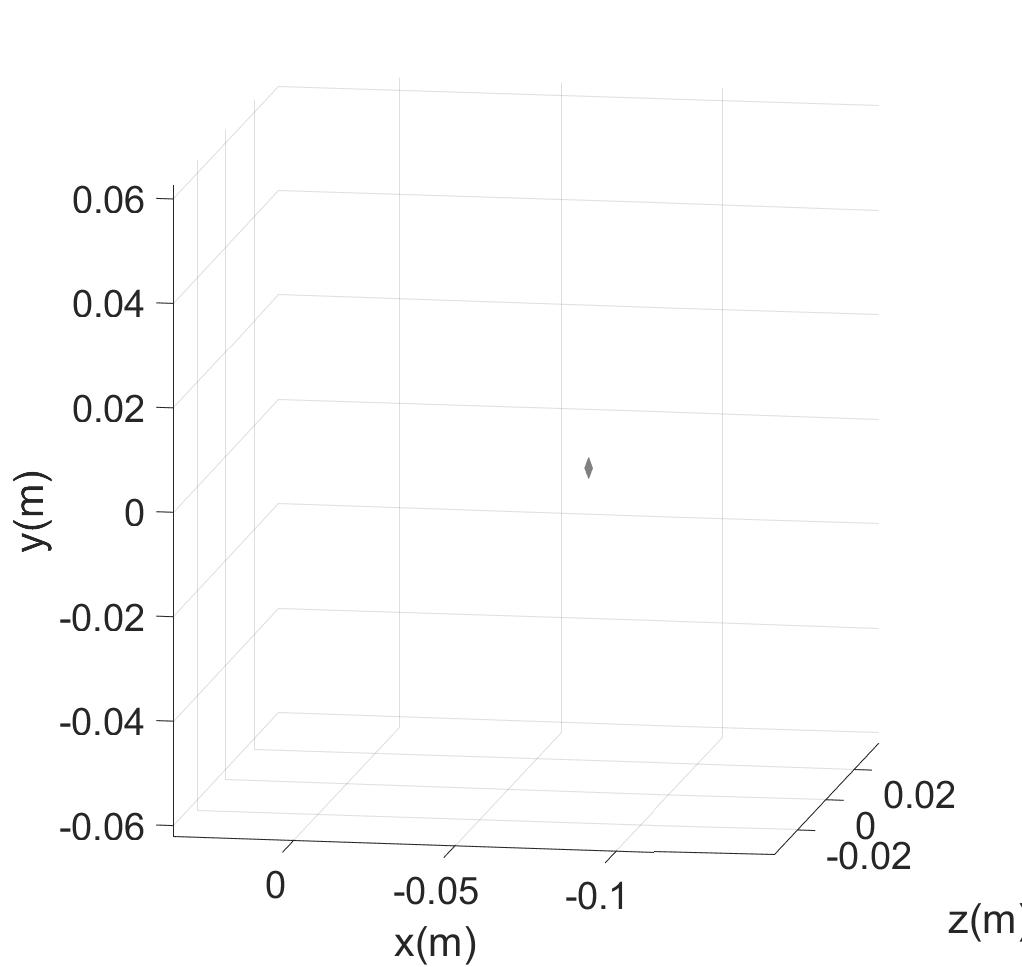
\includegraphics[width=1\linewidth]{../MatlabResults/CSAR_PSF_input}
				\caption{PSF Reflectivity Function}
				\label{fig:psf_in}
			\end{subfigure}%
			\begin{subfigure}{.5\linewidth}
				\label{fig:psf_out}
				\centering
				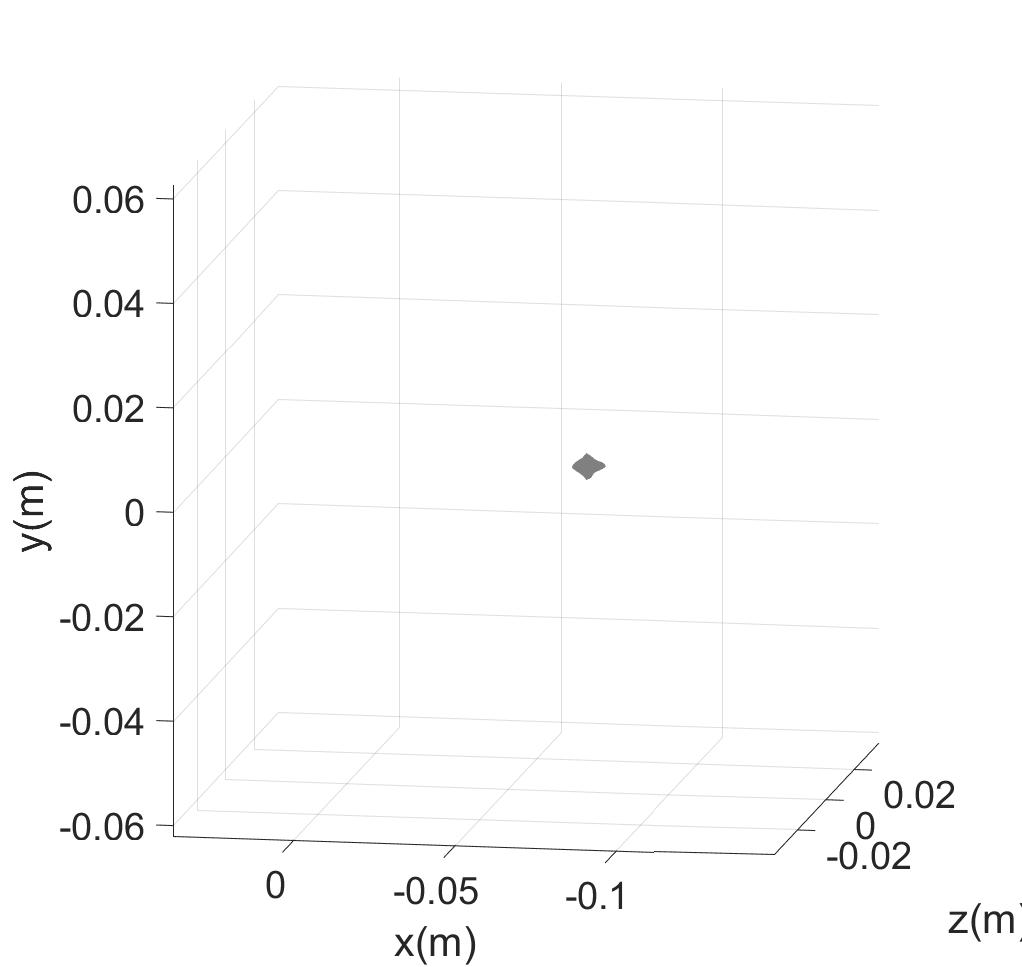
\includegraphics[width=1\linewidth]{../MatlabResults/CSAR_PSF_output}
				\caption{Reconstructed 3-D PSF}
			\end{subfigure}
			\begin{subfigure}{.5\linewidth}
				\label{fig:psf_xy}
				\centering
				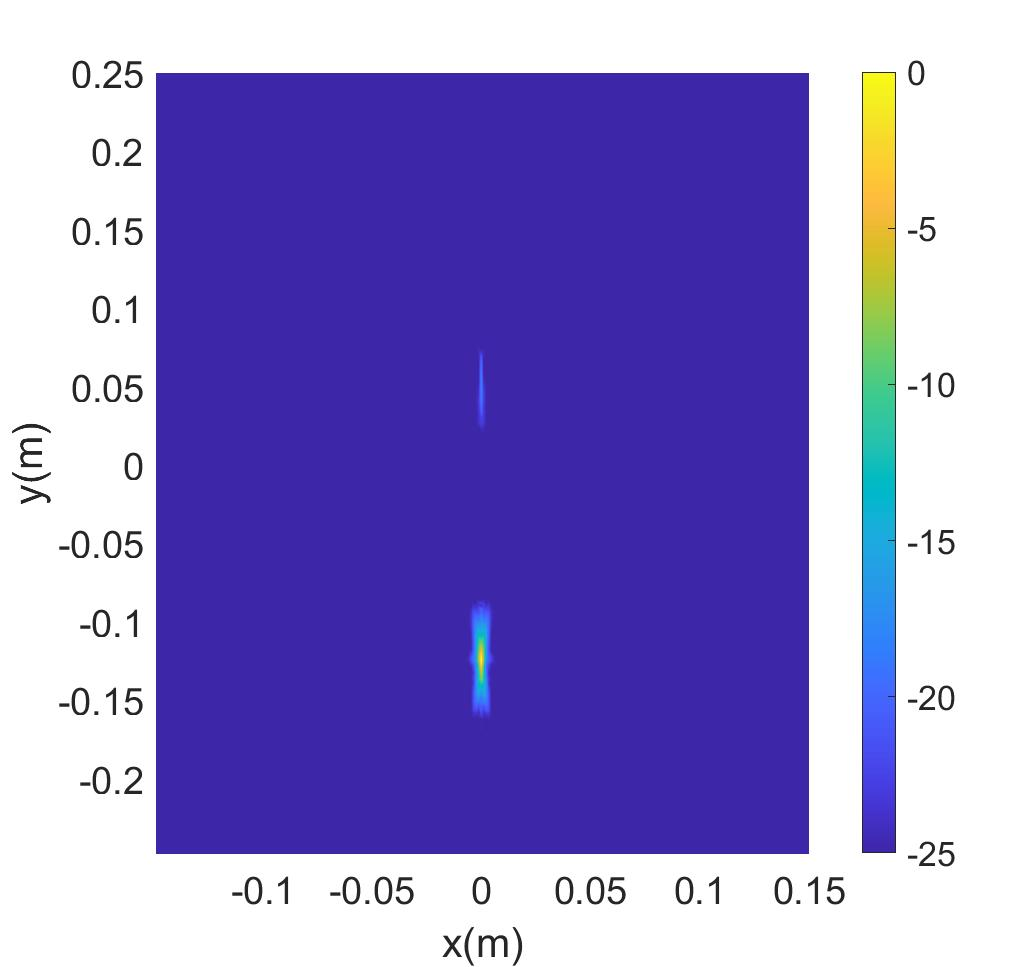
\includegraphics[width=1\linewidth]{../MatlabResults/CSAR_PSFxy}
				\caption{2-D x-y PSF (dB)}
			\end{subfigure}%
			\begin{subfigure}{.5\linewidth}
				\label{fig:psf_xz}
				\centering
				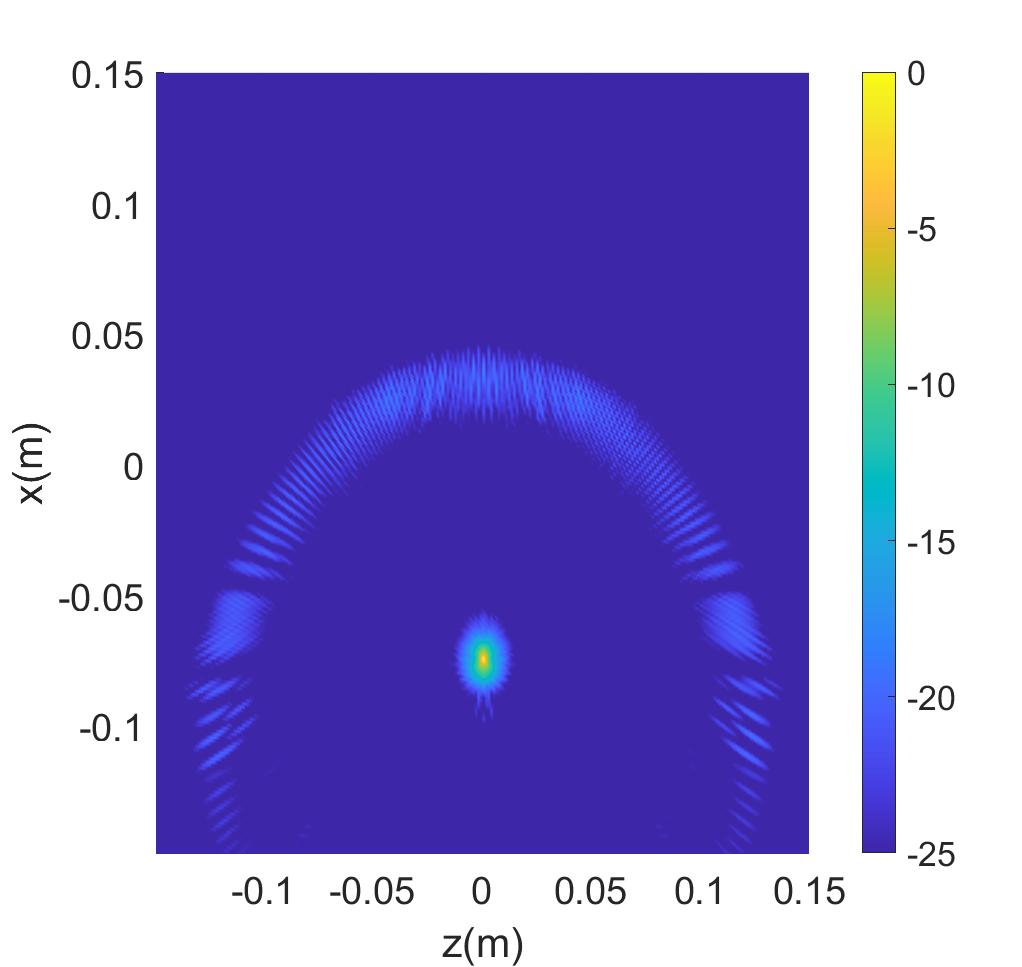
\includegraphics[width=1\linewidth]{../MatlabResults/CSAR_PSFxz}
				\caption{2-D x-z PSF (dB)}
			\end{subfigure}
			\begin{subfigure}{.5\linewidth}
				\label{fig:psf_yz}
				\centering
				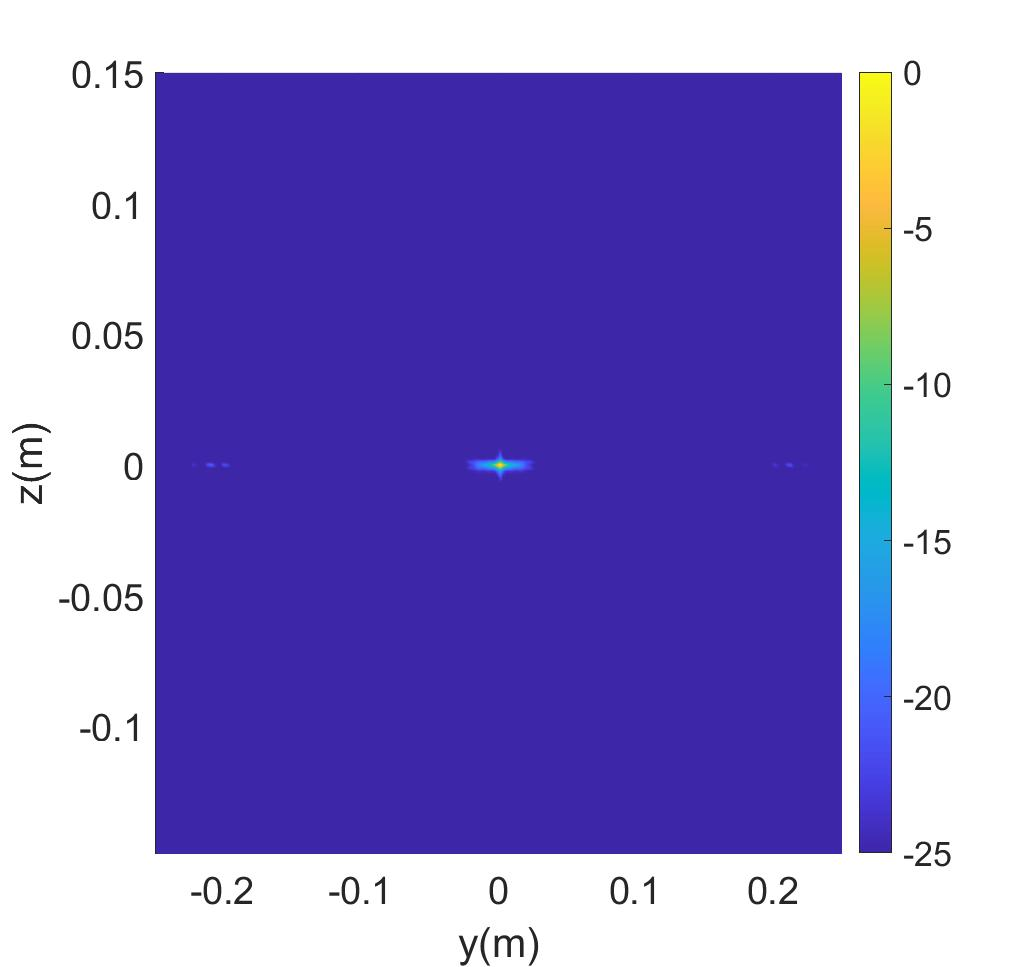
\includegraphics[width=1\linewidth]{../MatlabResults/CSAR_PSFyz}
				\caption{2-D y-z PSF (dB)}
			\end{subfigure}
			\caption{3-D input off-center point spread reflectivity function (a), 3-D output reconstructed PSF (b), 2-D vertical vs. cross range PSF (c), 2-D range vs. cross range PSF (d), 2-D range vs. vertical PSF (e)}
			\label{fig:psf}
		\end{figure}
	
		Discussion on the 2-D PSF slices
		
		\subsection{3D Points}
		%%************************************************************************************
		Additionally, to verify the algorithm in simulation, as set of points in a 3-D grid are generated and their echo signal is simulated. The algorithm again effectively reconstructs the images producing a nearly perfect duplicate of the input reflectivity function. 
		
		\begin{figure} [h]
			\begin{subfigure}{.5\linewidth}
				\centering
				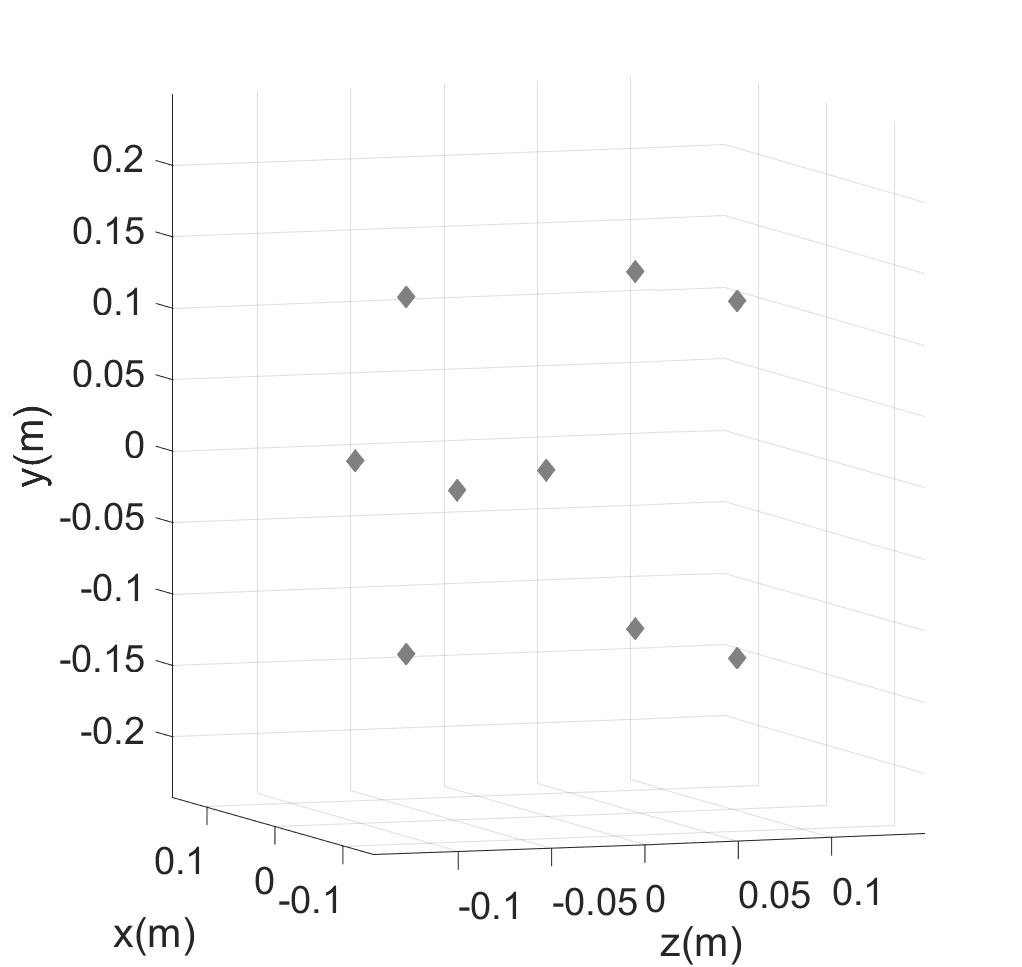
\includegraphics[width=1\linewidth]{../MatlabResults/CSAR_Grid3D_input}
				\caption{Reflectivity Function}
				\label{fig:grid3D_in}
			\end{subfigure}%
			\begin{subfigure}{.5\linewidth}
				\label{fig:grid3D_out}
				\centering
				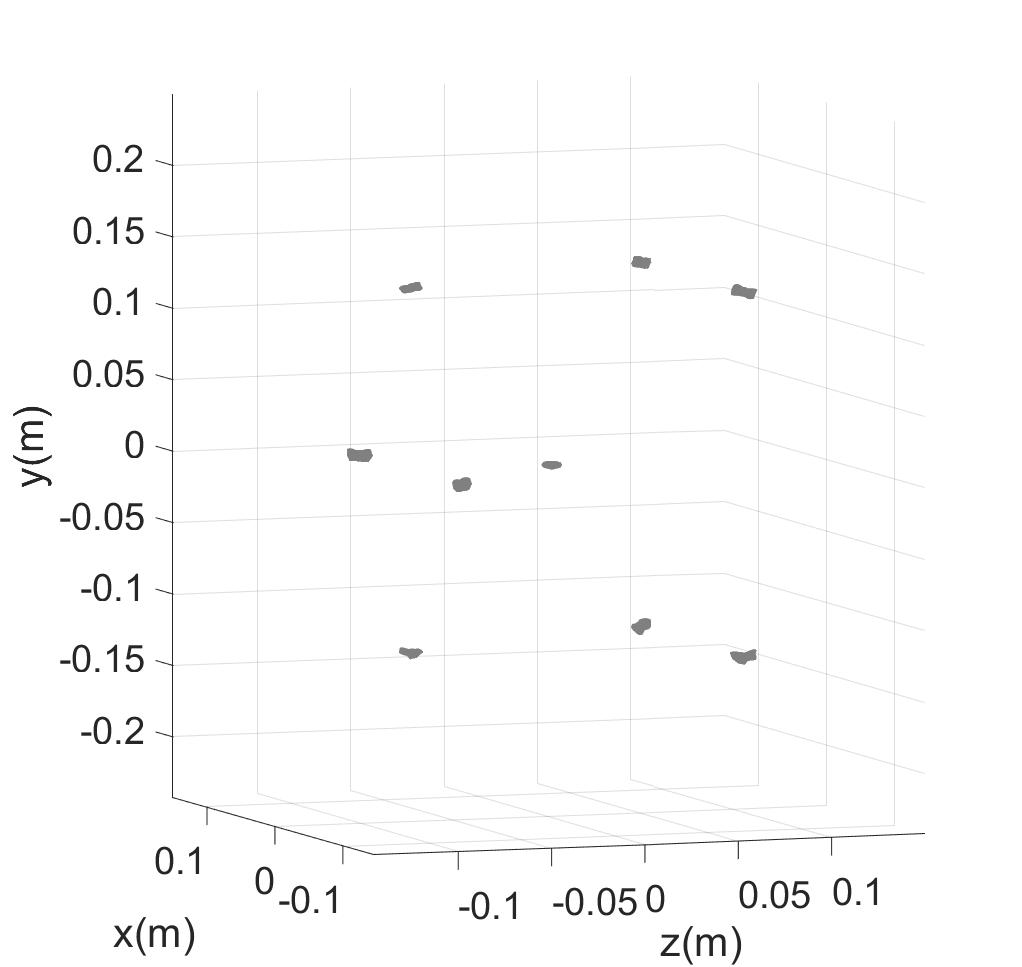
\includegraphics[width=1\linewidth]{../MatlabResults/CSAR_Grid3D_output}
				\caption{Reconstructed Image}
			\end{subfigure}
			\caption{3-D input grid of points reflectivity function (a), 3-D output reconstructed image (b)}
		\end{figure}
	
		With successful verification of the algorithm in simulation, a custom prototype R-ISAR scanner is built to experimentally capture data and test the algorithm's image quality on real echo data.
		
		\section{Experimental Setup}
		\label{sec:experimental_setup}
		%%************************************************************************************
		
		A cylindrical aperture is synthesized by mechanically moving a linear MIMO array continuously along a vertical track pattern, and rotating the target as shown in Fig.~\ref{fig:MIMO_R_ISAR_System_Configuration}. The system consists of Texas Instruments (TI) IWR1443-Boost, mmWave-Devpack, and TSW1400 \cite{TI:mmWave} mounted on a 2-D vertical and horizontal scanner as shown in Figure \ref{fig:scanner}. For this application, only the vertical motion is used. The scanned object is mounted on rotator. All mechanical motions are controlled by stepper drivers and embedded microcontrollers. The entire setup is controlled by a custom MATLAB graphical user interface (GUI), shown in Figure \ref{fig:matlab_gui}. 
		
		\begin{figure} [h]
			\begin{subfigure}{.5\linewidth}
				\centering
				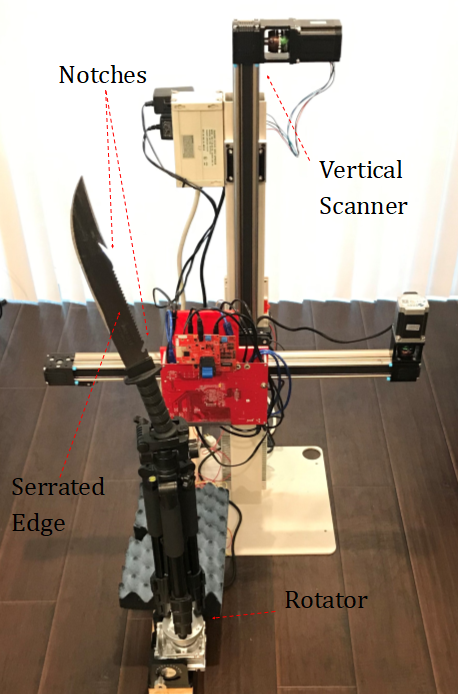
\includegraphics[width=1\linewidth]{../Figures/Scanner Photos/RSAR Scanner}
				\caption{Custom Prototype Scanner}
				\label{fig:scanner}
			\end{subfigure}%
			\begin{subfigure}{.5\linewidth}
				\centering
				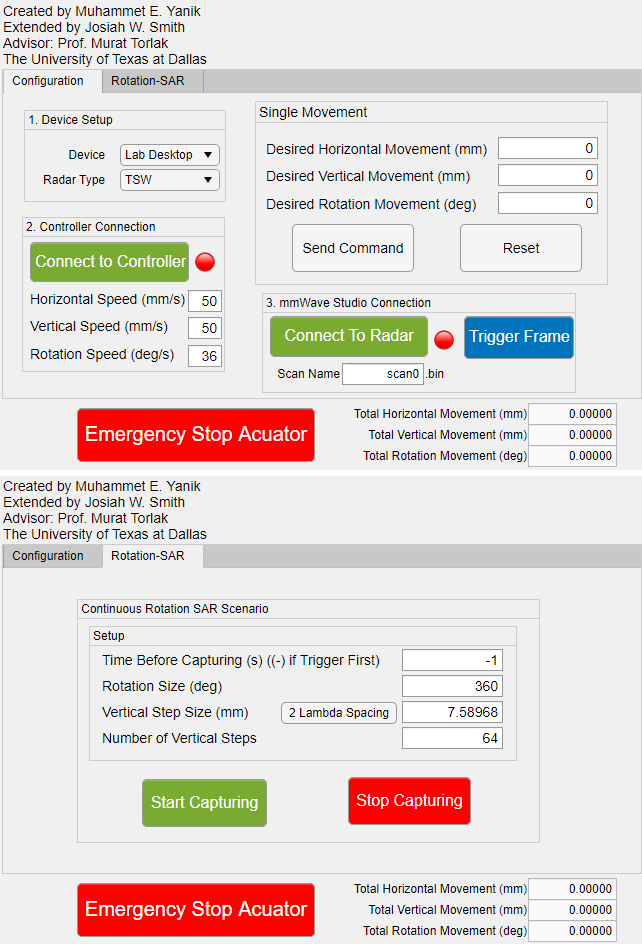
\includegraphics[width=1\linewidth]{../Figures/MATLAB RSAR GUI 2}
				\caption{MATLAB GUI}
				\label{fig:matlab_gui}
			\end{subfigure}
			\caption{Rotation-ISAR Scanner and MATLAB GUI}
		\end{figure}
		
		
		%%************************************************************************************
		\section{Imaging Results}
		\label{sec:imaging_results}
		%%************************************************************************************
		The 2-D vertical and rotational scan is performed by the prototype scanner. The large knife shown in Figure \ref{fig:scanner} is mounted to the rotator at an angle and scanned. Note the knife's notches and serrated edge. First, a scan is conducted using only a single channel and 
		
		\subsection{SISO Imaging Results}
		
		In the first experiment, a single transceiver pair is used to simulate a full-duplex SISO transceiver. Since the MIMO virtual array consists of 8 equally spaced virtual elements spanning $2\lambda$, the SISO scan will have a vertical spacing of $\lambda/4$ and will require 512 vertical captures to replicate the MIMO scan. All other parameters will remain the same, as shown in table \ref{table_SISO_radar_parameters}.
		
		\begin{table} [h]
			\caption{SISO Radar Parameters}
			\centering
			\begin{tabular}{c c c c c c c}
				\hline
				$R_0$ & $\Delta \theta$ & $\theta_{max}$ & $N_y$ & $\Delta y$ & B & $f_c$  \\ [0.5ex] 
				\hline\hline
				0.25 m & $0.036^{\circ}$ & $360^{\circ}$ & 512 & $\lambda/4$ & 4 GHz & 79 GHz \\ 
				\hline
			\end{tabular}
			\label{table_SISO_radar_parameters}
		\end{table}
	
		Once the scan is complete, the proposed MIMO R-ISAR 3-D holographic imaging algorithm is computed to reconstruct the 3-D target. 3-D volume rendering and maximum intensity profile (MIP) images are shown in Figure \ref{fig:knife_SISO}. As expected, the knife is easily visible, along with its notches and serrated edge. The entire scan took nearly two and a half hours to complete. By exploiting the nature of the MIMO virtual array, this scanning time can be drastically reduced. The algorithm proposed in Section \ref{sec:3D_mimo_algorithm} allows for this drastic reduction in scanning time without increasing the computational complexity of the image reconstruction algorithm. 
		
		\begin{figure} [h]
			\begin{subfigure}{.5\linewidth}
				\centering
				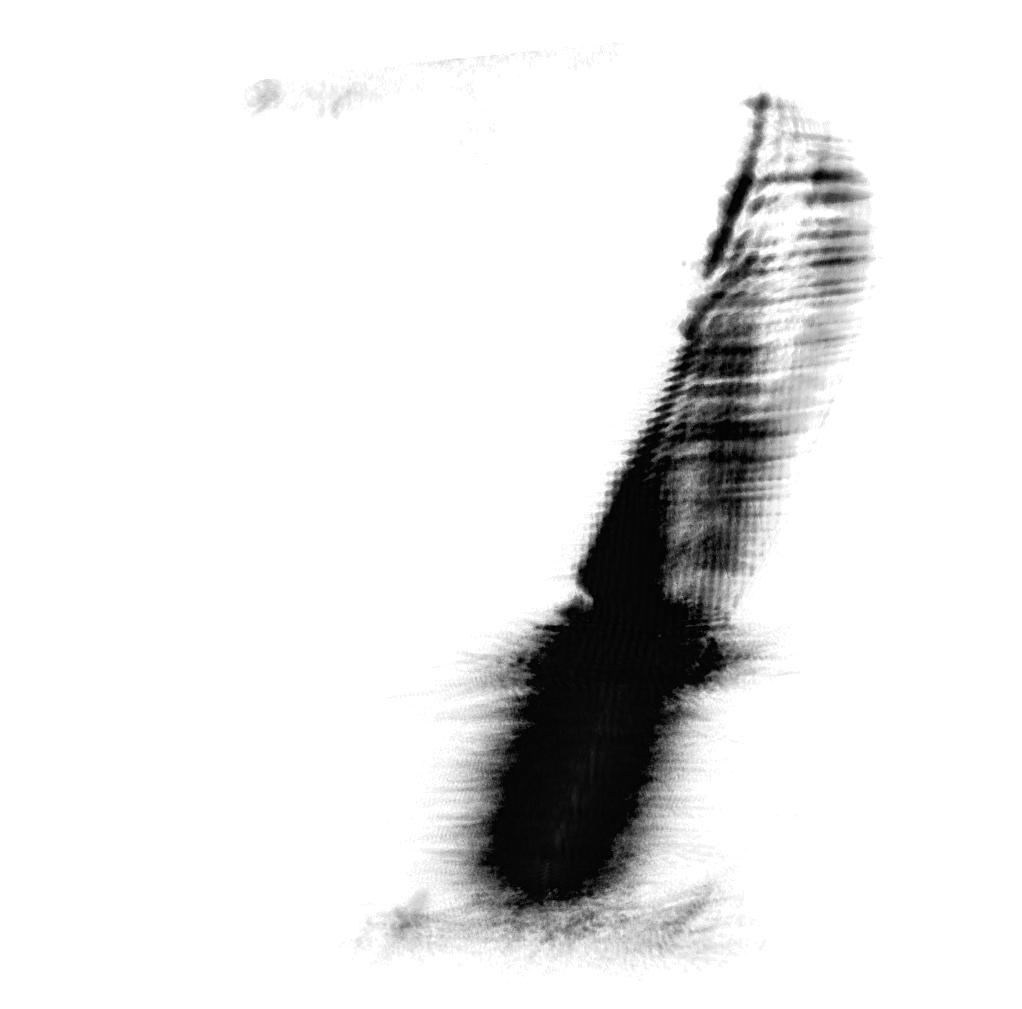
\includegraphics[width=1\linewidth]{../MatlabResults/knife_SISO_vr}
				\caption{Volume Rendering}
				\label{fig:knife_SISO_vr}
			\end{subfigure}%
			\begin{subfigure}{.5\linewidth}
				\centering
				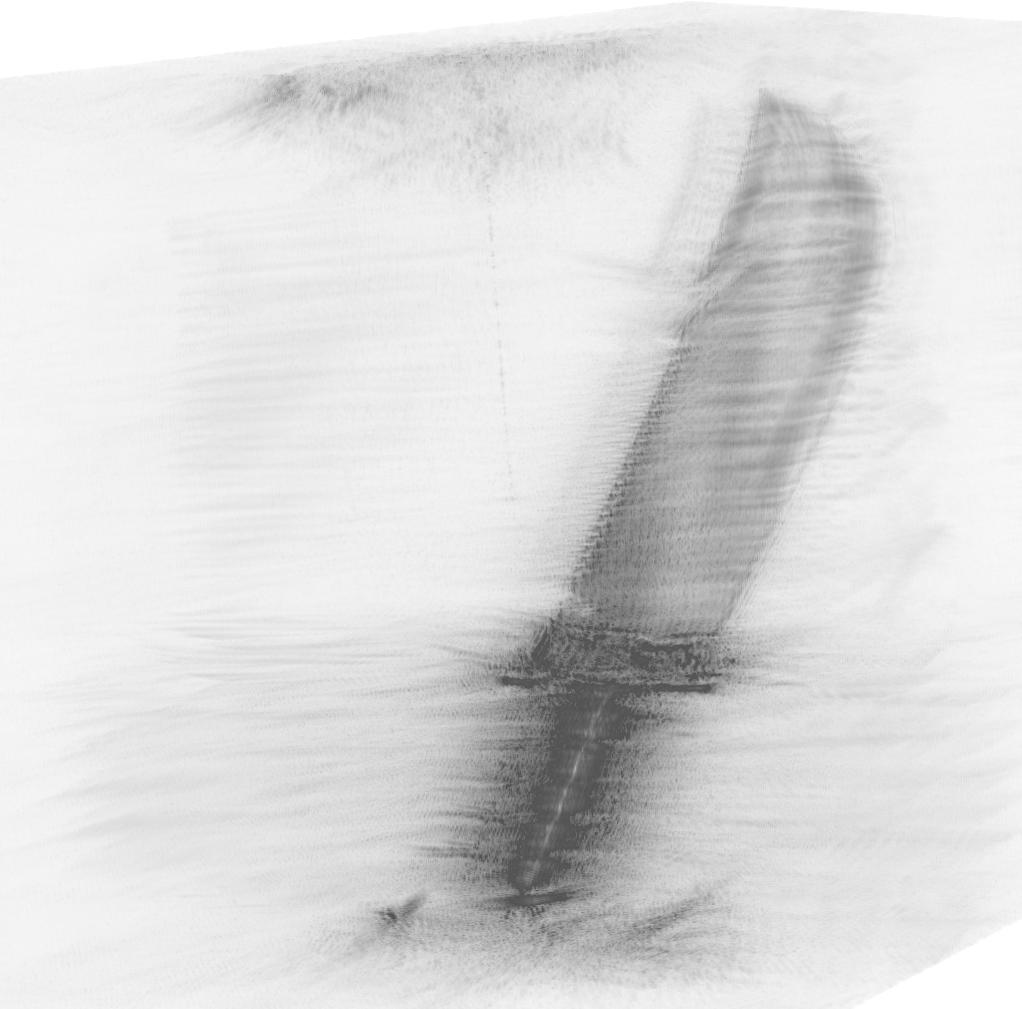
\includegraphics[width=1\linewidth]{../MatlabResults/knife_SISO_mip}
				\caption{Maximum Intensity Profile}
				\label{fig:knife_SISO_mip}
			\end{subfigure}
			\caption{SISO Reconstructed Image of Knife}
			\label{fig:knife_SISO}
		\end{figure}
		
		\subsection{MIMO Imaging Results}
		
		Now, the knife is scanned again, this time using all 2 Tx and 4 Tx antennas on the TI IWR1443-Boost. Before the multistatic-to-monostatic conversion and subsequent image reconstruction algorithm, the array calibration technique described in \cite{Yanik:NearFieldMIMOSAR} is employed to calibrate the phase of the echo signal and mitigate instrument delay. Then, the calibrated echo data is processed by the proposed R-ISAR MIMO 3-D holographic imaging algorithm and a high-resolution 3-D image is produced. Again, 3-D renderings are included below, in Figure \ref{fig:knife_MIMO}. The MIMO scan only took less than twenty minutes to complete, a significant reduction in comparison to the SISO scan.
		
		\begin{figure} [h]
			\begin{subfigure}{.5\linewidth}
				\centering
				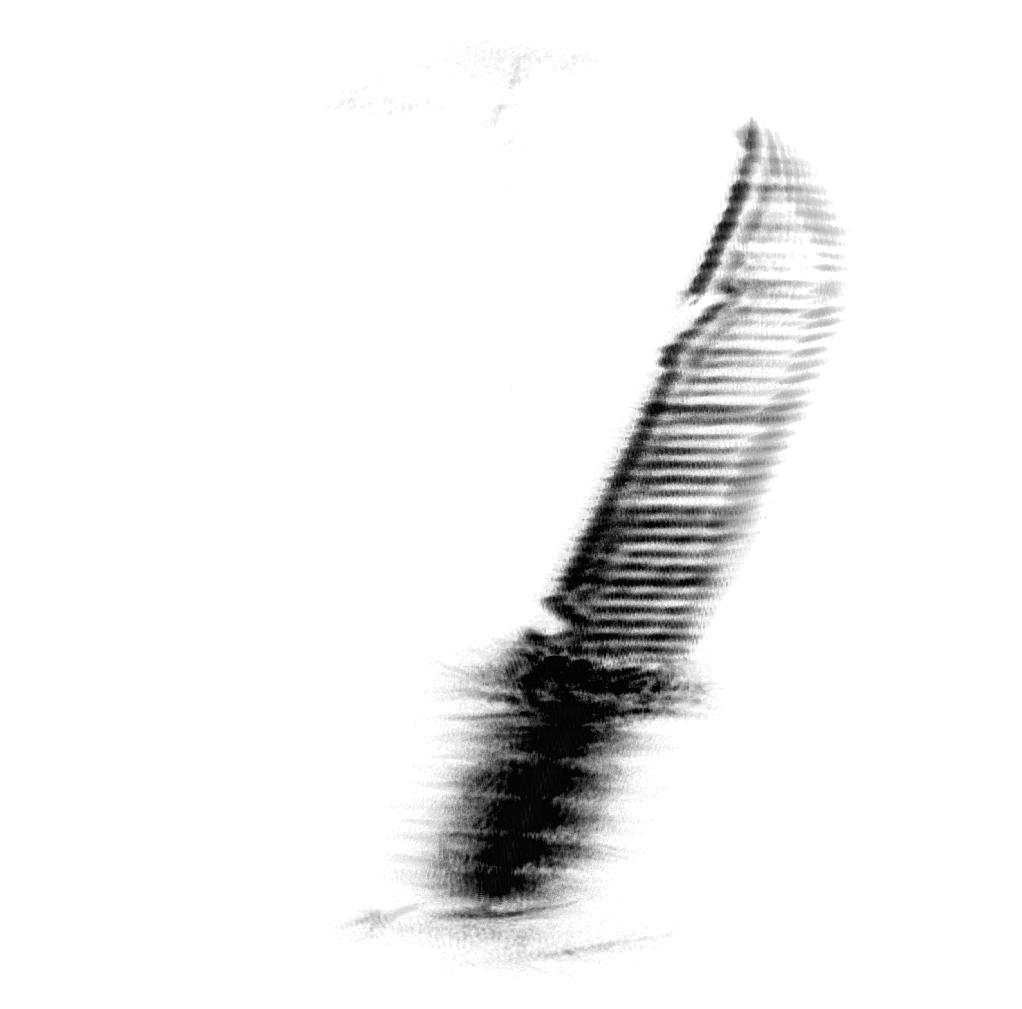
\includegraphics[width=1\linewidth]{../MatlabResults/knife_MIMO_vr}
				\caption{Volume Rendering}
				\label{fig:knife_MIMO_vr}
			\end{subfigure}%
			\begin{subfigure}{.5\linewidth}
				\centering
				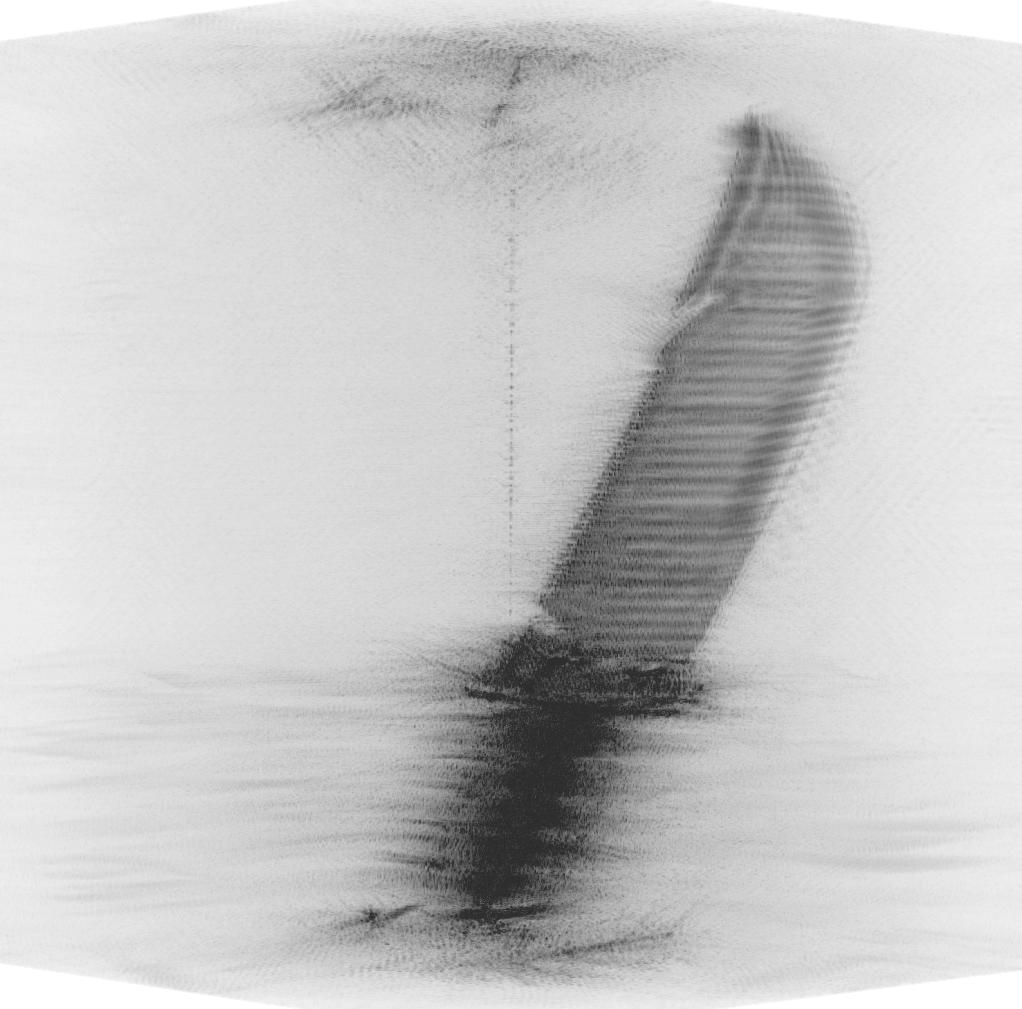
\includegraphics[width=1\linewidth]{../MatlabResults/knife_MIMO_mip}
				\caption{Maximum Intensity Profile}
				\label{fig:knife_MIMO_mip}
			\end{subfigure}
			\caption{MIMO Reconstructed Image of Knife}
			\label{fig:knife_MIMO}
		\end{figure}
	
		Examining both the SISO and MIMO images qualitatively, the image quality of the MIMO image appears to be the same, if not better, than that of the SISO scan. In fact, some artifacts at the top of the knife blade are visible in the horizontal domain of the SISO MIP image that are not visible in the MIMO image. This is likely do to a minor misalignment error in the rotational scan due to the large number of scans required for the SISO scan. These artifacts are likely not found in the MIMO scan since an eighth of the scans are required. By using the algorithm proposed in this paper, we were able to drastically reduce the scanning time while maintaining the computational efficiency of the SISO-based algorithms.
		
		\begin{table} [h]
			\caption{\label{table_scanning_times}Scanning Times}
			\centering
			\begin{tabular}{c c}
				\hline
				SISO Scanning Time & MIMO Scanning Time  \\ [0.5ex] 
				\hline
			    1032 (s) & 8202 (s) \\
				\hline
			\end{tabular}
		\end{table}
				
		%%************************************************************************************
		\section{Conclusion}
		\label{Sec_conclusion}
		%%************************************************************************************
		In this paper, we derived an efficient MIMO rotational-ISAR 3-D holographic imaging algorithm based on the single pixel polar formatting algorithm and multistatic-to-monostatic conversion. The algorithm successfully pairs the scanning efficiency of MIMO systems with the computational efficiency of SISO reconstruction algorithms. Additionally, we developed a complete, robust 3-D imaging system consisting of a vertically scanned MIMO radar and a rotator to rotate the target object. Our system fully integrates scanning scenario setup, data collection and calibration, algorithm implementation, and image inspection for a complete, efficient 3-D holographic imaging platform. Using this prototype system, high-resolution images are captured to demonstrated the effectiveness of this system for 3-D scene reconstruction and verify the MIMO R-ISAR algorithm's performance in comparison to its SISO counterpart. The algorithm and system demonstrate high-performance near-field imaging using MIMO rotational inverse synthetic radar radar.
		
		
		%%************************************************************************************
		\section*{Acknowledgment}
		%%************************************************************************************
		This work is supported by Semiconductor Research Corporation (SRC) task 2712.029 through The University of Texas at Dallas' Texas Analog Center of Excellence (TxACE).
		
		\bibliography{MIMO_ISAR_RadarConf20_Paper}
		\bibliographystyle{IEEEtran}
		
	\end{document}
